\section{Conditional prediction and sustained deviation}\label{sec:conditional}
The preceding experiments motivate a more specific question: how much can a predictor use observations to correct nominal-model error before that correction also weakens evidence of an unauthorized trajectory? A separate execution of RAPT~\cite{rapt} examines this issue. It is a transferred detector-core experiment, not a reproduction of the original humanoid study or a test of a claimed recovery guarantee.

\subsection{A fixed detector on exposed simulations}
The released model uses a residual encoder, a gated recurrent unit and Gaussian mean/variance outputs. We retain the author architecture and training loop, with batch size 32, one CPU thread and 100 epochs. Nine Q1 episodes from task K13 provide training; nine M13 episodes select the checkpoint by normal-development negative log likelihood; nine L13 episodes calibrate the released gates after checkpoint selection. Each population contains unchanged operation and two authorized-change conditions over three noise seeds. The selected checkpoint is epoch 14. A completed epoch budget does not imply convergence: development loss deteriorates later in this run. Observations are joint positions and velocities, and inputs include protected desired motion rather than the original humanoid observation/action interface.

For the frozen exploratory replay, this single checkpoint scores all 36 already exposed Q1 episodes from the contextual campaign. It detects 9 of 24 interventions and misses 15, with 5,175 alarms among 70,800 eligible benign points (7.309\%). Both declared model-only and hybrid modes give identical decisions. The detector is inactive on 9,448 of 10,689 physically outside-tolerance points. All six persistent-offset final quarters are inactive, covering 747 outside-tolerance points. The L19 cases react initially and later become inactive; the S19 cases are already below threshold early. No mode is selected after seeing these outcomes. Earlier ARX references have different commissioning histories, so their scores do not form a matched-training superiority comparison with this RAPT run.

\subsection{Separating prediction error from predicted variance}
The released channel score is
\begin{equation}
 \ell_{t,j}=(y_{t,j}-\mu_{t,j})^2\exp(-\nu_{t,j}),
 \label{eq:raptdecomposition}
\end{equation}
where $y$ is training-standardized and $\nu$ is predicted log variance. The training objective includes a log-variance term that is absent from this released score. Both mean and variance depend on observation history. A falling score alone therefore does not identify which component changed, or why.

A further no-fit replay saves both components without changing inputs, weights or calibration. All 518,400 channel-score values over 129,600 rows match the earlier output exactly; 126,000 rows are eligible after warmup. On positive-score support,
\begin{equation}
 \overline{\log\ell}=\overline{\log(y-\mu)^2}-\overline{\nu}.
\end{equation}
First-to-last quarter differences are computed separately within each channel. All 36 episodes and all conditions are retained in the execution record; no zero squared-error or score entries were excluded from these summaries. Figure~\ref{fig:decomposition} shows the persistent-offset contrasts that motivated the diagnostic.

\begin{figure*}[t]\centering
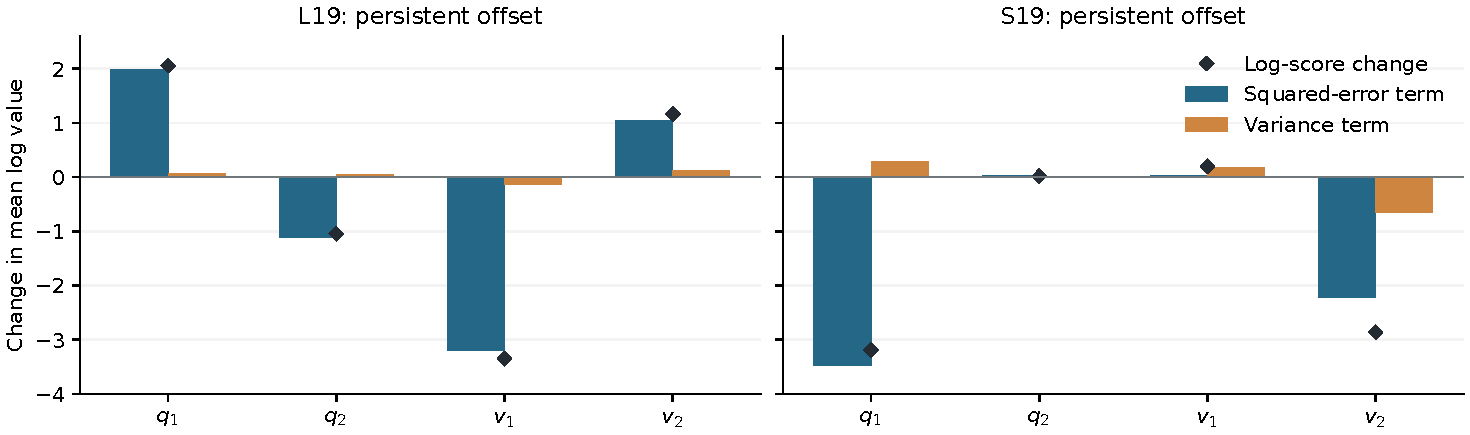
\includegraphics[width=0.91\textwidth]{figures/score_decomposition.pdf}
\caption{Exploratory decomposition of persistent-offset channel scores. Bars average each episode's last-minus-first quarter mean-log difference across three noise seeds. The numerator and negative log-variance terms add to the channel log-score change. They do not add to the max-over-gates detector risk. All position/velocity channels for both tasks are shown; the cases were already exposed before this diagnostic.}\label{fig:decomposition}
\end{figure*}

L19 position channel $q_1$ has an increasing mean log squared error ($+1.9838$), while the mean log squared error of its velocity channel $v_1$ decreases ($-3.2055$). For S19 $q_1$, the numerator decreases by $3.4826$, but decreasing variance partly opposes the score decline. These results exclude a uniform explanation based on all persistent position errors shrinking, or on variance inflation alone. They do not identify recurrence, immediate observation conditioning, phase, task transfer or calibration as the cause. Network parameters remain fixed during replay. The diagnostic adds visibility to an existing result; it supplies neither fresh attack confirmation nor evidence that a proposed replacement works.
